
%% bare_conf.tex
%% V1.3
%% 2007/01/11
%% by Michael Shell
%% See:
%% http://www.michaelshell.org/
%% for current contact information.
%%
%% This is a skeleton file demonstrating the use of IEEEtran.cls
%% (requires IEEEtran.cls version 1.7 or later) with an IEEE conference paper.
%%
%% Support sites:
%% http://www.michaelshell.org/tex/ieeetran/
%% http://www.ctan.org/tex-archive/macros/latex/contrib/IEEEtran/
%% and
%% http://www.ieee.org/

%%*************************************************************************
%% Legal Notice:
%% This code is offered as-is without any warranty either expressed or
%% implied; without even the implied warranty of MERCHANTABILITY or
%% FITNESS FOR A PARTICULAR PURPOSE! 
%% User assumes all risk.
%% In no event shall IEEE or any contributor to this code be liable for
%% any damages or losses, including, but not limited to, incidental,
%% consequential, or any other damages, resulting from the use or misuse
%% of any information contained here.
%%
%% All comments are the opinions of their respective authors and are not
%% necessarily endorsed by the IEEE.
%%
%% This work is distributed under the LaTeX Project Public License (LPPL)
%% ( http://www.latex-project.org/ ) version 1.3, and may be freely used,
%% distributed and modified. A copy of the LPPL, version 1.3, is included
%% in the base LaTeX documentation of all distributions of LaTeX released
%% 2003/12/01 or later.
%% Retain all contribution notices and credits.
%% ** Modified files should be clearly indicated as such, including  **
%% ** renaming them and changing author support contact information. **
%%
%% File list of work: IEEEtran.cls, IEEEtran_HOWTO.pdf, bare_adv.tex,
%%                    bare_conf.tex, bare_jrnl.tex, bare_jrnl_compsoc.tex
%%*************************************************************************

% *** Authors should verify (and, if needed, correct) their LaTeX system  ***
% *** with the testflow diagnostic prior to trusting their LaTeX platform ***
% *** with production work. IEEE's font choices can trigger bugs that do  ***
% *** not appear when using other class files.                            ***
% The testflow support page is at:
% http://www.michaelshell.org/tex/testflow/



% Note that the a4paper option is mainly intended so that authors in
% countries using A4 can easily print to A4 and see how their papers will
% look in print - the typesetting of the document will not typically be
% affected with changes in paper size (but the bottom and side margins will).
% Use the testflow package mentioned above to verify correct handling of
% both paper sizes by the user's LaTeX system.
%
% Also note that the "draftcls" or "draftclsnofoot", not "draft", option
% should be used if it is desired that the figures are to be displayed in
% draft mode.
%
\documentclass[conference]{IEEEtran}
% Add the compsoc option for Computer Society conferences.
%
% If IEEEtran.cls has not been installed into the LaTeX system files,
% manually specify the path to it like:
% \documentclass[conference]{../sty/IEEEtran}





% Some very useful LaTeX packages include:
% (uncomment the ones you want to load)


% *** MISC UTILITY PACKAGES ***
%
%\usepackage{ifpdf}
% Heiko Oberdiek's ifpdf.sty is very useful if you need conditional
% compilation based on whether the output is pdf or dvi.
% usage:
% \ifpdf
%   % pdf code
% \else
%   % dvi code
% \fi
% The latest version of ifpdf.sty can be obtained from:
% http://www.ctan.org/tex-archive/macros/latex/contrib/oberdiek/
% Also, note that IEEEtran.cls V1.7 and later provides a builtin
% \ifCLASSINFOpdf conditional that works the same way.
% When switching from latex to pdflatex and vice-versa, the compiler may
% have to be run twice to clear warning/error messages.






% *** CITATION PACKAGES ***
%
%\usepackage{cite}
% cite.sty was written by Donald Arseneau
% V1.6 and later of IEEEtran pre-defines the format of the cite.sty package
% \cite{} output to follow that of IEEE. Loading the cite package will
% result in citation numbers being automatically sorted and properly
% "compressed/ranged". e.g., [1], [9], [2], [7], [5], [6] without using
% cite.sty will become [1], [2], [5]--[7], [9] using cite.sty. cite.sty's
% \cite will automatically add leading space, if needed. Use cite.sty's
% noadjust option (cite.sty V3.8 and later) if you want to turn this off.
% cite.sty is already installed on most LaTeX systems. Be sure and use
% version 4.0 (2003-05-27) and later if using hyperref.sty. cite.sty does
% not currently provide for hyperlinked citations.
% The latest version can be obtained at:
% http://www.ctan.org/tex-archive/macros/latex/contrib/cite/
% The documentation is contained in the cite.sty file itself.






% *** GRAPHICS RELATED PACKAGES ***
%
\ifCLASSINFOpdf
\usepackage[pdftex]{graphicx}
  % declare the path(s) where your graphic files are
\graphicspath{{./images/}}
  % and their extensions so you won't have to specify these with
  % every instance of \includegraphics
\DeclareGraphicsExtensions{.jpg,.png}
\else
  % or other class option (dvipsone, dvipdf, if not using dvips). graphicx
  % will default to the driver specified in the system graphics.cfg if no
  % driver is specified.
  % \usepackage[dvips]{graphicx}
  % declare the path(s) where your graphic files are
  % \graphicspath{{../eps/}}
  % and their extensions so you won't have to specify these with
  % every instance of \includegraphics
  % \DeclareGraphicsExtensions{.eps}
\fi
% graphicx was written by David Carlisle and Sebastian Rahtz. It is
% required if you want graphics, photos, etc. graphicx.sty is already
% installed on most LaTeX systems. The latest version and documentation can
% be obtained at: 
% http://www.ctan.org/tex-archive/macros/latex/required/graphics/
% Another good source of documentation is "Using Imported Graphics in
% LaTeX2e" by Keith Reckdahl which can be found as epslatex.ps or
% epslatex.pdf at: http://www.ctan.org/tex-archive/info/
%
% latex, and pdflatex in dvi mode, support graphics in encapsulated
% postscript (.eps) format. pdflatex in pdf mode supports graphics
% in .pdf, .jpeg, .png and .mps (metapost) formats. Users should ensure
% that all non-photo figures use a vector format (.eps, .pdf, .mps) and
% not a bitmapped formats (.jpeg, .png). IEEE frowns on bitmapped formats
% which can result in "jaggedy"/blurry rendering of lines and letters as
% well as large increases in file sizes.
%
% You can find documentation about the pdfTeX application at:
% http://www.tug.org/applications/pdftex





% *** MATH PACKAGES ***
%
%\usepackage[cmex10]{amsmath}
% A popular package from the American Mathematical Society that provides
% many useful and powerful commands for dealing with mathematics. If using
% it, be sure to load this package with the cmex10 option to ensure that
% only type 1 fonts will utilized at all point sizes. Without this option,
% it is possible that some math symbols, particularly those within
% footnotes, will be rendered in bitmap form which will result in a
% document that can not be IEEE Xplore compliant!
%
% Also, note that the amsmath package sets \interdisplaylinepenalty to 10000
% thus preventing page breaks from occurring within multiline equations. Use:
%\interdisplaylinepenalty=2500
% after loading amsmath to restore such page breaks as IEEEtran.cls normally
% does. amsmath.sty is already installed on most LaTeX systems. The latest
% version and documentation can be obtained at:
% http://www.ctan.org/tex-archive/macros/latex/required/amslatex/math/





% *** SPECIALIZED LIST PACKAGES ***
%
%\usepackage{algorithmic}
% algorithmic.sty was written by Peter Williams and Rogerio Brito.
% This package provides an algorithmic environment fo describing algorithms.
% You can use the algorithmic environment in-text or within a figure
% environment to provide for a floating algorithm. Do NOT use the algorithm
% floating environment provided by algorithm.sty (by the same authors) or
% algorithm2e.sty (by Christophe Fiorio) as IEEE does not use dedicated
% algorithm float types and packages that provide these will not provide
% correct IEEE style captions. The latest version and documentation of
% algorithmic.sty can be obtained at:
% http://www.ctan.org/tex-archive/macros/latex/contrib/algorithms/
% There is also a support site at:
% http://algorithms.berlios.de/index.html
% Also of interest may be the (relatively newer and more customizable)
% algorithmicx.sty package by Szasz Janos:
% http://www.ctan.org/tex-archive/macros/latex/contrib/algorithmicx/




% *** ALIGNMENT PACKAGES ***
%
%\usepackage{array}
% Frank Mittelbach's and David Carlisle's array.sty patches and improves
% the standard LaTeX2e array and tabular environments to provide better
% appearance and additional user controls. As the default LaTeX2e table
% generation code is lacking to the point of almost being broken with
% respect to the quality of the end results, all users are strongly
% advised to use an enhanced (at the very least that provided by array.sty)
% set of table tools. array.sty is already installed on most systems. The
% latest version and documentation can be obtained at:
% http://www.ctan.org/tex-archive/macros/latex/required/tools/


%\usepackage{mdwmath}
%\usepackage{mdwtab}
% Also highly recommended is Mark Wooding's extremely powerful MDW tools,
% especially mdwmath.sty and mdwtab.sty which are used to format equations
% and tables, respectively. The MDWtools set is already installed on most
% LaTeX systems. The lastest version and documentation is available at:
% http://www.ctan.org/tex-archive/macros/latex/contrib/mdwtools/


% IEEEtran contains the IEEEeqnarray family of commands that can be used to
% generate multiline equations as well as matrices, tables, etc., of high
% quality.


%\usepackage{eqparbox}
% Also of notable interest is Scott Pakin's eqparbox package for creating
% (automatically sized) equal width boxes - aka "natural width parboxes".
% Available at:
% http://www.ctan.org/tex-archive/macros/latex/contrib/eqparbox/





% *** SUBFIGURE PACKAGES ***
%\usepackage[tight,footnotesize]{subfigure}
% subfigure.sty was written by Steven Douglas Cochran. This package makes it
% easy to put subfigures in your figures. e.g., "Figure 1a and 1b". For IEEE
% work, it is a good idea to load it with the tight package option to reduce
% the amount of white space around the subfigures. subfigure.sty is already
% installed on most LaTeX systems. The latest version and documentation can
% be obtained at:
% http://www.ctan.org/tex-archive/obsolete/macros/latex/contrib/subfigure/
% subfigure.sty has been superceeded by subfig.sty.



%\usepackage[caption=false]{caption}
%\usepackage[font=footnotesize]{subfig}
% subfig.sty, also written by Steven Douglas Cochran, is the modern
% replacement for subfigure.sty. However, subfig.sty requires and
% automatically loads Axel Sommerfeldt's caption.sty which will override
% IEEEtran.cls handling of captions and this will result in nonIEEE style
% figure/table captions. To prevent this problem, be sure and preload
% caption.sty with its "caption=false" package option. This is will preserve
% IEEEtran.cls handing of captions. Version 1.3 (2005/06/28) and later 
% (recommended due to many improvements over 1.2) of subfig.sty supports
% the caption=false option directly:
%\usepackage[caption=false,font=footnotesize]{subfig}
%
% The latest version and documentation can be obtained at:
% http://www.ctan.org/tex-archive/macros/latex/contrib/subfig/
% The latest version and documentation of caption.sty can be obtained at:
% http://www.ctan.org/tex-archive/macros/latex/contrib/caption/




% *** FLOAT PACKAGES ***
%
%\usepackage{fixltx2e}
% fixltx2e, the successor to the earlier fix2col.sty, was written by
% Frank Mittelbach and David Carlisle. This package corrects a few problems
% in the LaTeX2e kernel, the most notable of which is that in current
% LaTeX2e releases, the ordering of single and double column floats is not
% guaranteed to be preserved. Thus, an unpatched LaTeX2e can allow a
% single column figure to be placed prior to an earlier double column
% figure. The latest version and documentation can be found at:
% http://www.ctan.org/tex-archive/macros/latex/base/



\usepackage{stfloats}
% stfloats.sty was written by Sigitas Tolusis. This package gives LaTeX2e
% the ability to do double column floats at the bottom of the page as well
% as the top. (e.g., "\begin{figure*}[!b]" is not normally possible in
% LaTeX2e). It also provides a command:
%\fnbelowfloat
% to enable the placement of footnotes below bottom floats (the standard
% LaTeX2e kernel puts them above bottom floats). This is an invasive package
% which rewrites many portions of the LaTeX2e float routines. It may not work
% with other packages that modify the LaTeX2e float routines. The latest
% version and documentation can be obtained at:
% http://www.ctan.org/tex-archive/macros/latex/contrib/sttools/
% Documentation is contained in the stfloats.sty comments as well as in the
% presfull.pdf file. Do not use the stfloats baselinefloat ability as IEEE
% does not allow \baselineskip to stretch. Authors submitting work to the
% IEEE should note that IEEE rarely uses double column equations and
% that authors should try to avoid such use. Do not be tempted to use the
% cuted.sty or midfloat.sty packages (also by Sigitas Tolusis) as IEEE does
% not format its papers in such ways.





% *** PDF, URL AND HYPERLINK PACKAGES ***
%
%\usepackage{url}
% url.sty was written by Donald Arseneau. It provides better support for
% handling and breaking URLs. url.sty is already installed on most LaTeX
% systems. The latest version can be obtained at:
% http://www.ctan.org/tex-archive/macros/latex/contrib/misc/
% Read the url.sty source comments for usage information. Basically,
% \url{my_url_here}.





% *** Do not adjust lengths that control margins, column widths, etc. ***
% *** Do not use packages that alter fonts (such as pslatex).         ***
% There should be no need to do such things with IEEEtran.cls V1.6 and later.
% (Unless specifically asked to do so by the journal or conference you plan
% to submit to, of course. )


% correct bad hyphenation here
\hyphenation{op-tical net-works semi-conduc-tor}


\begin{document}
%
% paper title
% can use linebreaks \\ within to get better formatting as desired
\title{Dual Block/Text Editing in Many Languages}


% author names and affiliations
% use a multiple column layout for up to three different
% affiliations
\author{\IEEEauthorblockN{D. Anthony Bau}
\IEEEauthorblockA{Phillips Exeter Academy\\
Exeter, New Hampshire 03833\\
Email: dbau@exeter.edu}
}

% conference papers do not typically use \thanks and this command
% is locked out in conference mode. If really needed, such as for
% the acknowledgment of grants, issue a \IEEEoverridecommandlockouts
% after \documentclass

% for over three affiliations, or if they all won't fit within the width
% of the page, use this alternative format:
% 
%\author{\IEEEauthorblockN{Michael Shell\IEEEauthorrefmark{1},
%Homer Simpson\IEEEauthorrefmark{2},
%James Kirk\IEEEauthorrefmark{3}, 
%Montgomery Scott\IEEEauthorrefmark{3} and
%Eldon Tyrell\IEEEauthorrefmark{4}}
%\IEEEauthorblockA{\IEEEauthorrefmark{1}School of Electrical and Computer Engineering\\
%Georgia Institute of Technology,
%Atlanta, Georgia 30332--0250\\ Email: see http://www.michaelshell.org/contact.html}
%\IEEEauthorblockA{\IEEEauthorrefmark{2}Twentieth Century Fox, Springfield, USA\\
%Email: homer@thesimpsons.com}
%\IEEEauthorblockA{\IEEEauthorrefmark{3}Starfleet Academy, San Francisco, California 96678-2391\\
%Telephone: (800) 555--1212, Fax: (888) 555--1212}
%\IEEEauthorblockA{\IEEEauthorrefmark{4}Tyrell Inc., 123 Replicant Street, Los Angeles, California 90210--4321}}




% use for special paper notices
%\IEEEspecialpapernotice{(Invited Paper)}




% make the title area
\maketitle


\begin{abstract}
%\boldmath
Droplet is new programming editor that can edit arbitrary code in a blocks-based environment. This paper presents Droplet's techniques for parsing and editing a wide variety of languages, including Python, Java, JavaScript, C, BASIC, and CoffeeScript. It presents a general framework for adapting Droplet to a new language, and discusses techniques for doing rudimentary type-checking and preserving order of operations while editing.

\end{abstract}
% IEEEtran.cls defaults to using nonbold math in the Abstract.
% This preserves the distinction between vectors and scalars. However,
% if the conference you are submitting to favors bold math in the abstract,
% then you can use LaTeX's standard command \boldmath at the very start
% of the abstract to achieve this. Many IEEE journals/conferences frown on
% math in the abstract anyway.

% no keywords




% For peer review papers, you can put extra information on the cover
% page as needed:
% \ifCLASSOPTIONpeerreview
% \begin{center} \bfseries EDICS Category: 3-BBND \end{center}
% \fi
%
% For peerreview papers, this IEEEtran command inserts a page break and
% creates the second title. It will be ignored for other modes.
\IEEEpeerreviewmaketitle



\section{Introduction}
Droplet is a new programming editor that edits text programs in a drag-and-drop blocks environment \cite{Droplet}. Drag-and-drop block languages such as Scratch and Blockly are accessible to learners: Scratch and Blockly are both popular, and Moskal, et al. found that Alice helped improve the attitudes of "at risk" students \cite{Moskal}.
Droplet was initially implemented with CoffeeScript and used with Pencilcode, a previously text-based environment \cite{Droplet}\cite{Pencilcode}. A similar tool was developed to work specifically with Grace, and was successful at teaching students to transition from blocks to text \cite{TiledGrace}.

This paper discusses preliminary work to generalize Droplet to several other text programming languages. In the 2013 National Secondary School Computer Science Surveys, Python, C++, Visual Basic, JavaScript, and Java each accounted for over 10\% of American high school introductory curricula \cite{CSTA}. A survey by Guo of university courses in 2014 found Python, Java, MATLAB, C, C++, and Scheme all made up significant portions of higher-level introductory courses \cite{Guo}. Here we report on our progress and findings extending the Droplet block editor to Java, C, Python, JavaScript, LOGO, and BASIC.

\section{Background}

\subsection{Droplet's Text-First Approach to Blocks}

\begin{figure*}[!t]
\centering
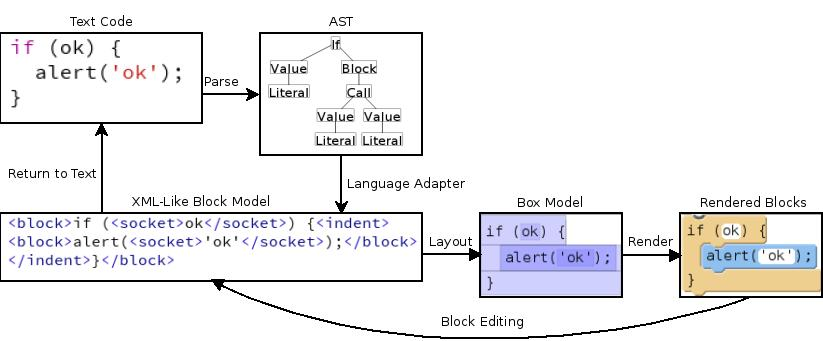
\includegraphics[width=5in]{image11.jpg}
\caption{Lifecycle of a Droplet Program}
\label{lifecycle}
\end{figure*}

\begin{figure}[!t]
\centering
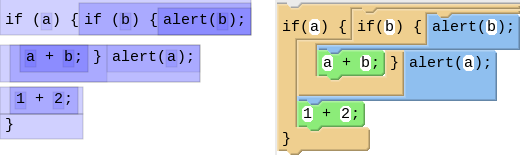
\includegraphics[width=2.5in]{image05.png}
\caption{Droplet Rendering Badly-Indented Text}
\label{bad_layout}
\end{figure}

\begin{figure}[!t]
\centering
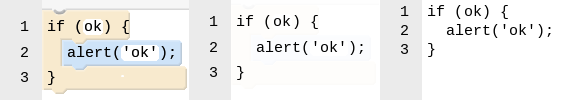
\includegraphics[width=2.5in]{image12.png}
\caption{Frames of Droplet's Block/Text Animation}
\label{anim}
\end{figure}

Droplet was built to bridge the gap between blocks and text. Droplet's primary guiding philosophy is that the text, not the blocks, are the primary data. Thus, Droplet programs begin and end their life as text. When Droplet opens a program file, it runs the program text through a language adapter and inserts markup which indicates where blocks should go and how they should be rendered. The user interacts with this rendering of the program, performing splice operations on the markup stream. During editing, the language mode may be called back to preserve precedence or dictate droppability rules. At the end of the editing session, the markup is simply discarded and a raw text program is generated again. Figure \ref{lifecycle} shows a typical Droplet editing session in JavaScript.

Droplet programs are frequently formatted to look like Scratch blocks when programs are indented properly. However, Droplet's renderer is able to render any text layout (Fig. \ref{bad_layout}).

Droplet will always lay out the text in the blocks as it appears in the source text. This is both to follow Droplet's text-first philosophy and to facilitate an animation between blocks and text (Fig. \ref{anim}).

\subsection{Live Reparsing}

\begin{figure}[!t]
\centering
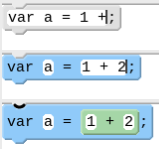
\includegraphics[width=1.5in]{livereparse.png}
\caption{Live Reparsing. Either of the top two configurations will become the bottom one.}
\label{livereparse}
\end{figure}

Droplet also has support for "handwritten" blocks and live reparsing, which blend text editing and block editing. When editing, a user can press the return key to get a blank line, in which they can type arbitrary code, which gets parsed and turned into blocks when complete. The user can also type arbitrary expressions into sockets in blocks, which get reparsed and turned into blocks when complete (Fig. \ref{livereparse}).

\subsection{The Droplet Markup Scheme}
Droplet has three types of markup entities: Blocks, Sockets, and Indents. Blocks are solid-colored, draggable ranges; Sockets are white, typeable, droppable ranges that can contain single Blocks; Indents are ranges that include multiple Blocks and render their children with interlocking tabs. All three node types can have arbitrary "classes" attached to them, which is simply a list of strings that the language mode assigns at parse time and can re-examine later.

Indents consume whitespace at the beginning of each line; this whitespace is removed from the text stream while editing. This is done so that drags can be interpreted as simple splice operations. The whitespace is reinserted using the Indent metadata when the raw text is regenerated. Each Indent has as metadata a prefix to add to each line; if any lines are misformatted and do not line up with the indent, those lines are flagged as exceptions and handled appropriately when the text is regenerated.

\section{Approach}
A new Droplet language mode must perform three tasks:
\begin{enumerate}
  \item Adding markup to a text program to describe rendering
  \item Handling droppability rules and preserving order of operations
  \item Facilitating live reparsing
\end{enumerate}

Droplet uses a variety of techniques to attempt to accomplish these for as many languages as possible. This paper presents a framework for traversing an arbitrary language AST, along with strategies for doing type-checking and order-of-operations preservation for unknown languages.

\subsection{The Parser Wrapper Layer}
All Droplet parsers output to the parser wrapper layer, which exists between the language mode and the editor. The wrapper layer provides universal fidelity and renderability guarantees.

A language mode must output Block, Socket, and Indent entities with associated location data. These can be outputted in any order, but each must be associated with a depth property that allows the entities to be sorted by depth in the program syntax tree. The parser wrapper layer recieves this output and the program text and inserts the markup into the text, consuming whitespace and flagging oddly-indented lines where necessary. If there is free-floating text after this has been done, the parser wrapper layer surrounds it with a draggable white block, so that the user can decide what to do with it (free-floating text on its own is immutable).

\subsection{General AST Traversal: The Droplet treewalker Framework}
In our work generalizing Droplet to new languages, we designed a treewalk framework that facilitates a standard AST traversal for generating Droplet's block-language markup. A parser wrapper using the Treewalker framework needs only to generate a parse tree in a unified format, and then dictate which node types should trigger each kind of event. The event types that must be denoted for each AST node are as follows:

Generating Droplet markup from an abstract syntax tree usually involves a depth-first AST traversal. The Droplet treewalker framework facilitates this. Five types of events can happen when a Droplet treewalker traversal encounters a node:
\begin{enumerate}
  \item indent
  \item paren
  \item merge
  \item block/socket
  \item socket terminal
\end{enumerate}

A \textbf{merge} event skips the node and proceeds directly to its children without adding a block boundary. If a node has exactly one child, it is automatically skipped regardless of how the mode was configured. An automatically skipped node, however, is recorded, and if a Block is generated, it is flagged as having the node type of all the skipped nodes. This facilitiates automatic rudimentary type-checking, as discussed in the ANTLR adapter section.

A \textbf{socket terminal} event makes a typable socket around a terminal token.

A \textbf{block/socket} event is the basic Droplet event, and is applicable to most AST nodes. Most nodes should become blocks in the output, so a Block is created. However, a Block cannot immediately have a Block parent (when the Block is removed, it must leave behind a Socket), so a Socket must be inserted directly around the Block.

An \textbf{indent} event generates an Indent node in the Droplet markup. Most languages do not have strict whitespace rules, so the indent depth of an Indent can sometimes be ambiguous. Unless other information is available, the indent depth is determined by majority count over all the lines in the range that are not within other Indent children. Indents exclude leading and trailing free text, as this is usually a non-operational marker like "\{" or "\}" that should properly belong to the indent's parent.

\begin{figure}[!t]
\centering
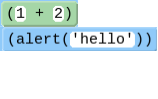
\includegraphics[width=1.5in]{parenparens.png}
\caption{Paren nodes. These nodes have different colors and metadata even though they are the same node in the AST.}
\label{paren_parens}
\end{figure}

A \textbf{paren} event uses the location data of a parent node but the classes and rendering information of a child node. This is necessary to properly handle parentheses and semicolons; for instance, in Figure \ref{paren_parens}, "(alert("hello"))" is colored blue but "(1 + 1)" is colored green, even though both are identical paren nodes. Adapters for languages that use semicolons may similarly wish to include the semicolon in a block that does not, in the AST, actually contain the semicolon.

\subsection{Strategies for Droppability}

\subsection{Strategies for Precedence}
In Droplet's hand-coded modes (CoffeeScript and JavaScript), precedence is handled with metadata on Blocks and Sockets. Each Block is assigned a precedence number based on its node type, and each Socket is assigned a precedence number based on its parent's node type. Whenever a drop occurs, Droplet calls back the language mode to see if parentheses need to be inserted or removed. The language mode compares precedence numbers, and, if necessary, modifies the block's leading and trailing text only (for instance, adding "(" prefix and ")" suffix) to preserve the order of operations. The same callback is also used for semicolons in block statements and commas in array literals. When called back, the language mode recieves the classes that it assigned at parse time, as well as the preceding and succeeding sibling nodes, and can thenceforth determine whether it needs to insert or remove a semicolon or a comma.

\subsection{Strategies for Live Reparsing}
If a parser, like ANTLR-generated parsers, exposes arbitrary parsing contexts, live reparsing reparses the closest parent using its node type, which will have been stored in the "classes" flag at parse time.

For parsers that do not expose arbitrary parsing contexts, Droplet simulates non-root parsing contexts by assigning a piece of metadata to each Block. This metadata is three strings: a prefix, a suffix, and an indent prefix. When parsing, Droplet concatenates the prefix, input string, and suffix, and parses (fully, so the output is a Droplet markup stream) it at the root context. It then scans forward in the generated markup stream to the end of the prefix. If there is a single Droplet markup entity (Block, Socket, or Indent) that starts at the end of the prefix and ends at the beginning of the suffix, it splices this entity out and uses it as the parse.

If the language mode fails to assign an appropriate parsing context, Droplet instead attempts to bubble the reparse up the parents of the nodes until parsing succeeds, ultimately attempting to reparse the entire document. If this fails, Droplet informs the user that they have made a syntax error by highlighting the socket in red.

\subsection{Integration with ANTLR}
The ANTLR framework extends the Droplet treewalker framework to format the ANTLR parse tree automatically. It also implements rudimentary type-checking and order-of-operations preservation methods. A configuration for an ANTLR mode is entirely declarative, consisting only of the node types that should trigger each type of treewalk event.

ANTLR modes do rudimentary type-checking by examining AST node types. Most frequently, Block/Socket pair events have two or more node types because of the first heuristic. The Socket is flagged as only the highest node (closest to the root), whlie the Block is flagged as all the node types. When checking for droppability, an ANTLR mode checks to see if the target Socket node type is any of the Block's node types. This guarantees that the result is always legal, although it also occasionally forbids legal combinations.

\begin{figure*}[!t]
\centering
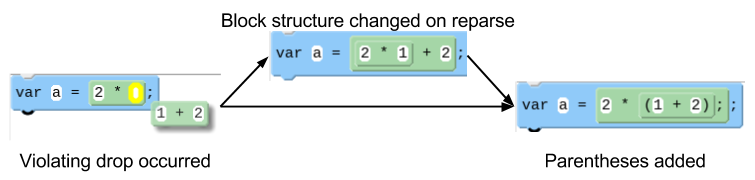
\includegraphics[width=5in]{autoparen.png}
\caption{Automatic Order of Operations by Reparsing}
\label{fig_sim}
\end{figure*}

ANTLR modes do not have any structured method for doing parenthesis and order-of-operations checking. To attempt to preserve order of operations, ANTLR modes instead attempt to place a node inside another node and immediately reparse. If the reparse changes the structure of the blocks, it is assumed that order-of-operations was broken, and parentheses are inserted.

\section{Results}
\begin{table}[!t]
  \renewcommand{\arraystretch}{1.3}
  \caption{Implemented Languages}
  \label{impl_lang}
  \centering
  \begin{tabular}{|c|c|c|c|}
    \hline
    CoffeeScript & CoffeeScript compiler & Hand-coded & 982\\
    \hline
    JavaScript & acorn.js & Hand-coded & 526\\
    \hline
    Python & Skulpt compiler & Treewalk framework & 81\\
    \hline
    Java & ANTLR & ANTLR framework & 44\\
    \hline
    C & ANTLR (C11 standard) & ANTLR framework & 42\\
    \hline
    Basic & ANTLR (jvmBasic grammar) & ANTLR framework & 28\\
    \hline
    Logo & ANTLR & ANTLR framework & 28\\
    \hline
  \end{tabular}
\end{table}

Three parsers have been written from custom parsers: CoffeeScript (using the CoffeeScript compiler), JavaScript (using acorn.js), and Python (using the Skulpt compiler). Five parsers have been written using ANTLR grammars: Java, C (from the C11 spec, without preprocessing directives), BASIC (using the jvmBasic grammar), Logo, and R. The adapter file for Python is less than 100 lines long, and configuration files for each of Java, C, BASIC, Logo, and R are less than 50 lines each. Each of these parsers is able to parse any valid program, and guarantees 100\% fidelity on all programs.

\section{Discussion}
The language modes implemented in this paper cover every non-visual imperative language in the NCSSCSS and all the most popular languages Guo found in his survey of university courses except MATLAB and Scheme. More importantly, however, the ANTLR and Droplet treewalker frameworks provide a way for additional languages to be implemented extremely quickly even if the implementer does not know the language.

\begin{thebibliography}{1}

\bibitem{Droplet}
  Bau, D. A. Droplet, A Blocks-Based Editor for Text Code. Journal of Computer Science in Colleges. 30, 6 (June 2015).
\bibitem{Moskal}
  Moskal B, Lurie D, and Cooper S. Evaluating the Effectiveness of a New Instructional Approach. Proceedings of the 35th SIGCSE Technical Symposium on Computer Science Education.
\bibitem{TiledGrace}
  Homer M. Combining Tiled and Textual Views of Code. in 2nd IEEE Working Conference on Software Visualization (Victoria, CA, 2014), IEEE, 1-4.
\bibitem{Pencilcode}
  Bau D, Bau D. A. A Preview of Pencil Code. Proceedings of the 2014 ACM Conference on Systems, Programming and Applications. (In press.)
\bibitem{CSTA}
  Computer Science Teachers Association. CSTA National Secondary School Computer Science Survey (2013). http://csta.acm.org/Research/sub/Projects/ResearchFiles/CSTASurvey13Results.pdf. Accessed Mar 14, 2015.
\bibitem{Guo}
  Guo, P. Python is Now the Most Popular Introductory Teaching Language at Top U.S. Universities. Communications of the ACM blog. http://cacm.acm.org/blogs/blog-cacm/176450-python-is-now-the-most-popular-introductory-teaching-language-at-top-us-universities/fulltext. Accessed Mar 14, 2015.


\end{thebibliography}

% that's all folks
\end{document}


